
\chapter{Introduction\label{ch:intro}}

Talk about the increasing use of quadcopters for a variety of uses.

Advantages of using quadcopters, disadvantages/difficulties.

Transition to the difficulties 

\section{Motivation}

\section{Current Acquisition Methods}

\subsection{Laser Scanners}
Laser rangefinder technology is the ``gold standard'' of 3D model acquisition in terms of quality. Modern scanners can produce sub millimeter accuracy, which make them a great choice for detailed digitization of statues. Combined with high-resolution photograph texture-mapping, very few techniques can match the precision and quality of these scans. The Digital Michelangelo Project showed the power and precision of laser scanners by scanning several different statues, including Michelangelo's David, to 1/4mm accuracy.\cite{Levoy}

\begin{figure}
\centering
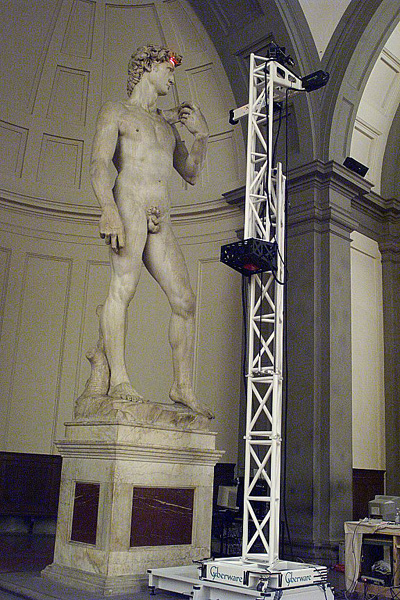
\includegraphics[height=200px]{../images/david_scan.jpg}
\caption{An example of a laser scanner setup used by the Digital Michelangelo Project \cite{Levoy}.}
\end{figure}

However, laser scanners do have several drawbacks. The equipment is extremely expensive, bulky, and fragile. The Michelangelo Project had to transport over 4 tons of equipment to Italy in order to produce their scans. Additionally, laser scans involve immense setup and can take many hours. The scan of David took over a thousand man-hours to scan and even more than that in post processing \cite{Levoy}.

\subsubsection{Multi-View Stereo}
Multi-view stereo uses a collection of 2D images to reconstruct a 3D object model. By viewing a single object from hundreds of different camera positions, a 3D model can be generated. Although this technique originally required precisely known camera coordinates, recent algorithms can produce a 3D model from an unordered collection of images with unknown camera positions, assuming that there is sufficient coverage. Existing software packages such as Bundler and Agisoft Photoscan can produce high-quality 3D reconstructions using these unordered image collections. \cite{bundler}\cite{photoscan}

The ability to use a collection of images without precise camera position information means that these 3D objects can be modeled substantially faster than with a laser scanner. With a smaller object, it is a relatively simple process to take pictures of the object from many different angles. However, for a larger object, such as a statue or building, the problem of gathering imagery becomes substantially more difficult.

\begin{figure}
\centering
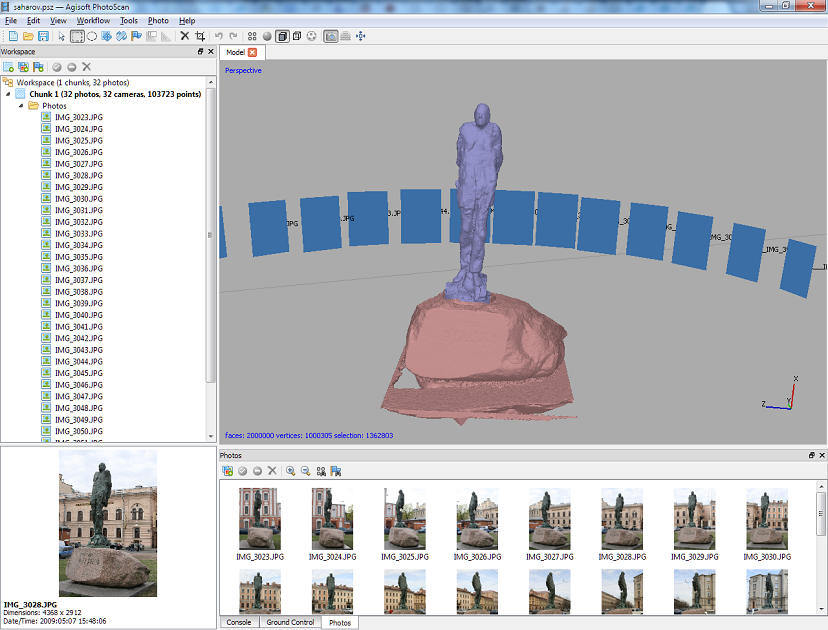
\includegraphics[height=200px]{../images/photoscan.png}
\caption{A 3D model of a statue generated by Agisoft Photoscan. Notice the derived camera planes encompassing the statue \cite{photoscan}.}
\end{figure}

\subsection{Problem Definition}
We look to create a system to capture imagery of large 3D objects for use in multi-view stereo software. This system has several requirements.

\begin{enumerate}
\item
\textbf{Low Cost}

The system should be substantially cheaper than laser scanning.

\item
\textbf{Easy to Use}

This system should be able to be deployed by users with minimal training. Additionally, the hardware should be off-the-shelf and easily accessible.

\item
\textbf{Complete Coverage}

The system must be able to capture images from a wide variety of positions, completely covering every part of the target object.

\item
\textbf{High Quality Imagery}

The system must produce sufficiently high resolution, non-blurry images for use in multi-view stereo software.

\end{enumerate}

\subsection{Proposed Solution}

We propose using low-cost autonomous quadcopters to gather imagery needed for use in multi-view stereo software. By flying a quadcopter with a mounted camera around the target object, we can quickly and thoroughly capture images of the target from a wide variety of positions. Using quadcopters has many advantages.

\begin{enumerate}
\item
Quadcopters can capture images from positions unreachable by ground-based cameras.

\item
By methodically flying around the target object at different altitudes, we can guarantee complete coverage of the target object.

\item
The imagery can be captured very quickly, on the order of a few minutes.

\item
Quadcopters are small, portable, and easily deployable.


\end{enumerate}

